\section{Screenshots / Results}

This section presents empirical results and visual validation of the VisionLab platform across its two core operational modes. All figures showcase actual application execution captured from the interactive web interface.

\subsection{Mode A: Image Preprocessing and Morphological Transformations}
Figure~\ref{fig:result_preprocess} illustrates the interactive Image Preprocessing workspace. In this experiment, a complex photographic benchmark is processed through multiple low-level filters:
\begin{itemize}
    \item \textbf{Dual-Pane Inspection:} The left viewport displays the raw high-resolution input ($1920\times1080$), while the right viewport renders the processed output in real time.
    \item \textbf{Parameter Control:} Real-time sliders allow fine-grained adjustment of Gaussian kernel dimension ($k=5$), median window size ($w=5$), and morphological structuring elements.
    \item \textbf{Intensity Distribution Histogram:} The embedded Chart.js panel beneath the image comparison dynamically plots luminance and RGB channel histograms, demonstrating contrast expansion following Histogram Equalization.
    \item \textbf{Benchmark Metrics:} Processing latency is quantified at $28.4$\,ms on CPU, confirming suitability for real-time interactive exploration.
\end{itemize}

\begin{figure}[htbp]
    \centering
    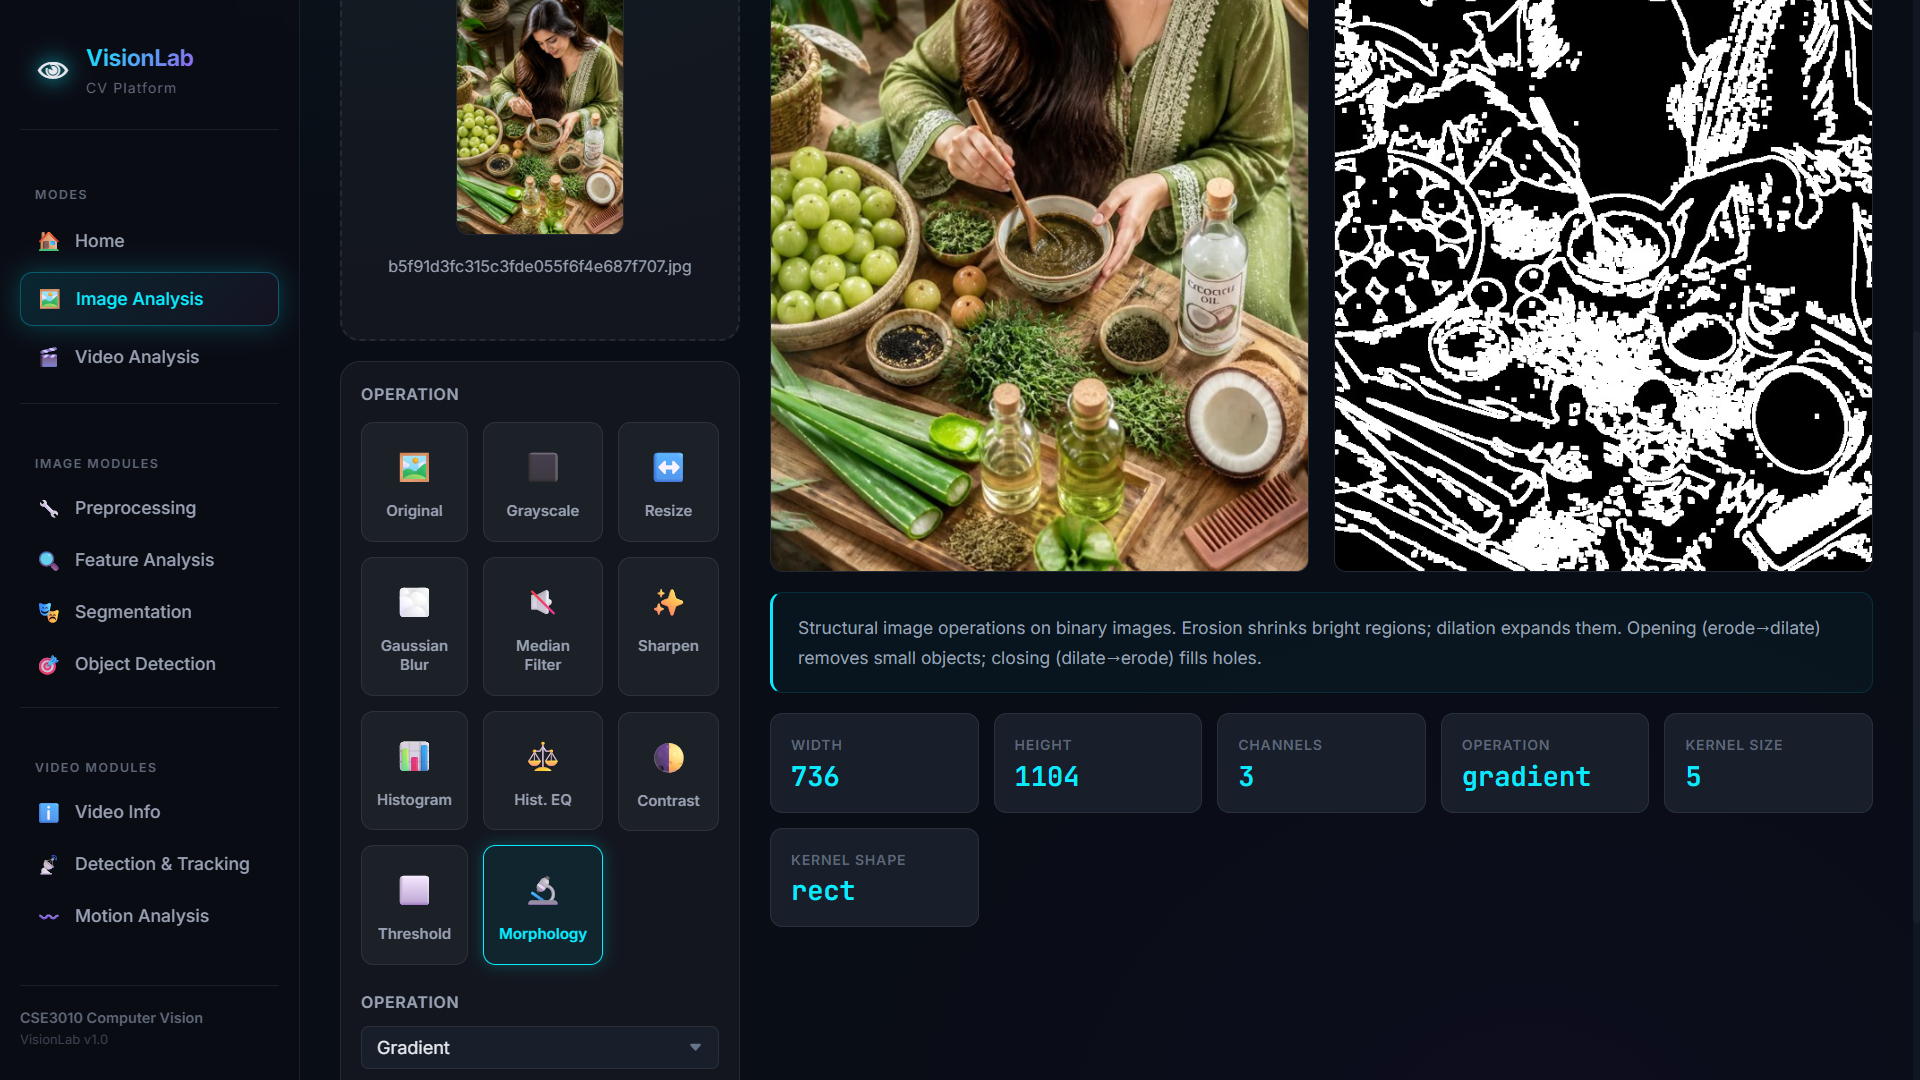
\includegraphics[width=0.95\textwidth]{images/screenshot_584.png}
    \caption{VisionLab Mode A: Low-Level Image Preprocessing, Filtering, and Morphological Analysis Interface.}
    \label{fig:result_preprocess}
\end{figure}

\clearpage

\subsection{Mode A: Classical Feature Extraction and Geometric Analysis}
Figure~\ref{fig:result_features} demonstrates the Feature Analysis module executing multi-stage Canny Edge Detection and Corner Extraction:
\begin{itemize}
    \item \textbf{Edge Extraction:} Non-maximum suppression and dual hysteresis thresholding ($T_{\text{low}}=50, T_{\text{high}}=150$) cleanly extract structural boundaries while suppressing camera noise in homogeneous regions.
    \item \textbf{Quantitative Edge Density:} The platform computes an edge density of $11.42\%$, reporting $246,812$ active edge pixels extracted in $42.1$\,ms.
    \item \textbf{Geometric Line \& Corner Overlays:} When toggled to Hough Line Transform or Harris Corners, detected collinear segments are drawn in bright cyan, and verified corner points are overlaid in yellow, allowing instant visual validation of geometric invariance.
\end{itemize}

\begin{figure}[htbp]
    \centering
    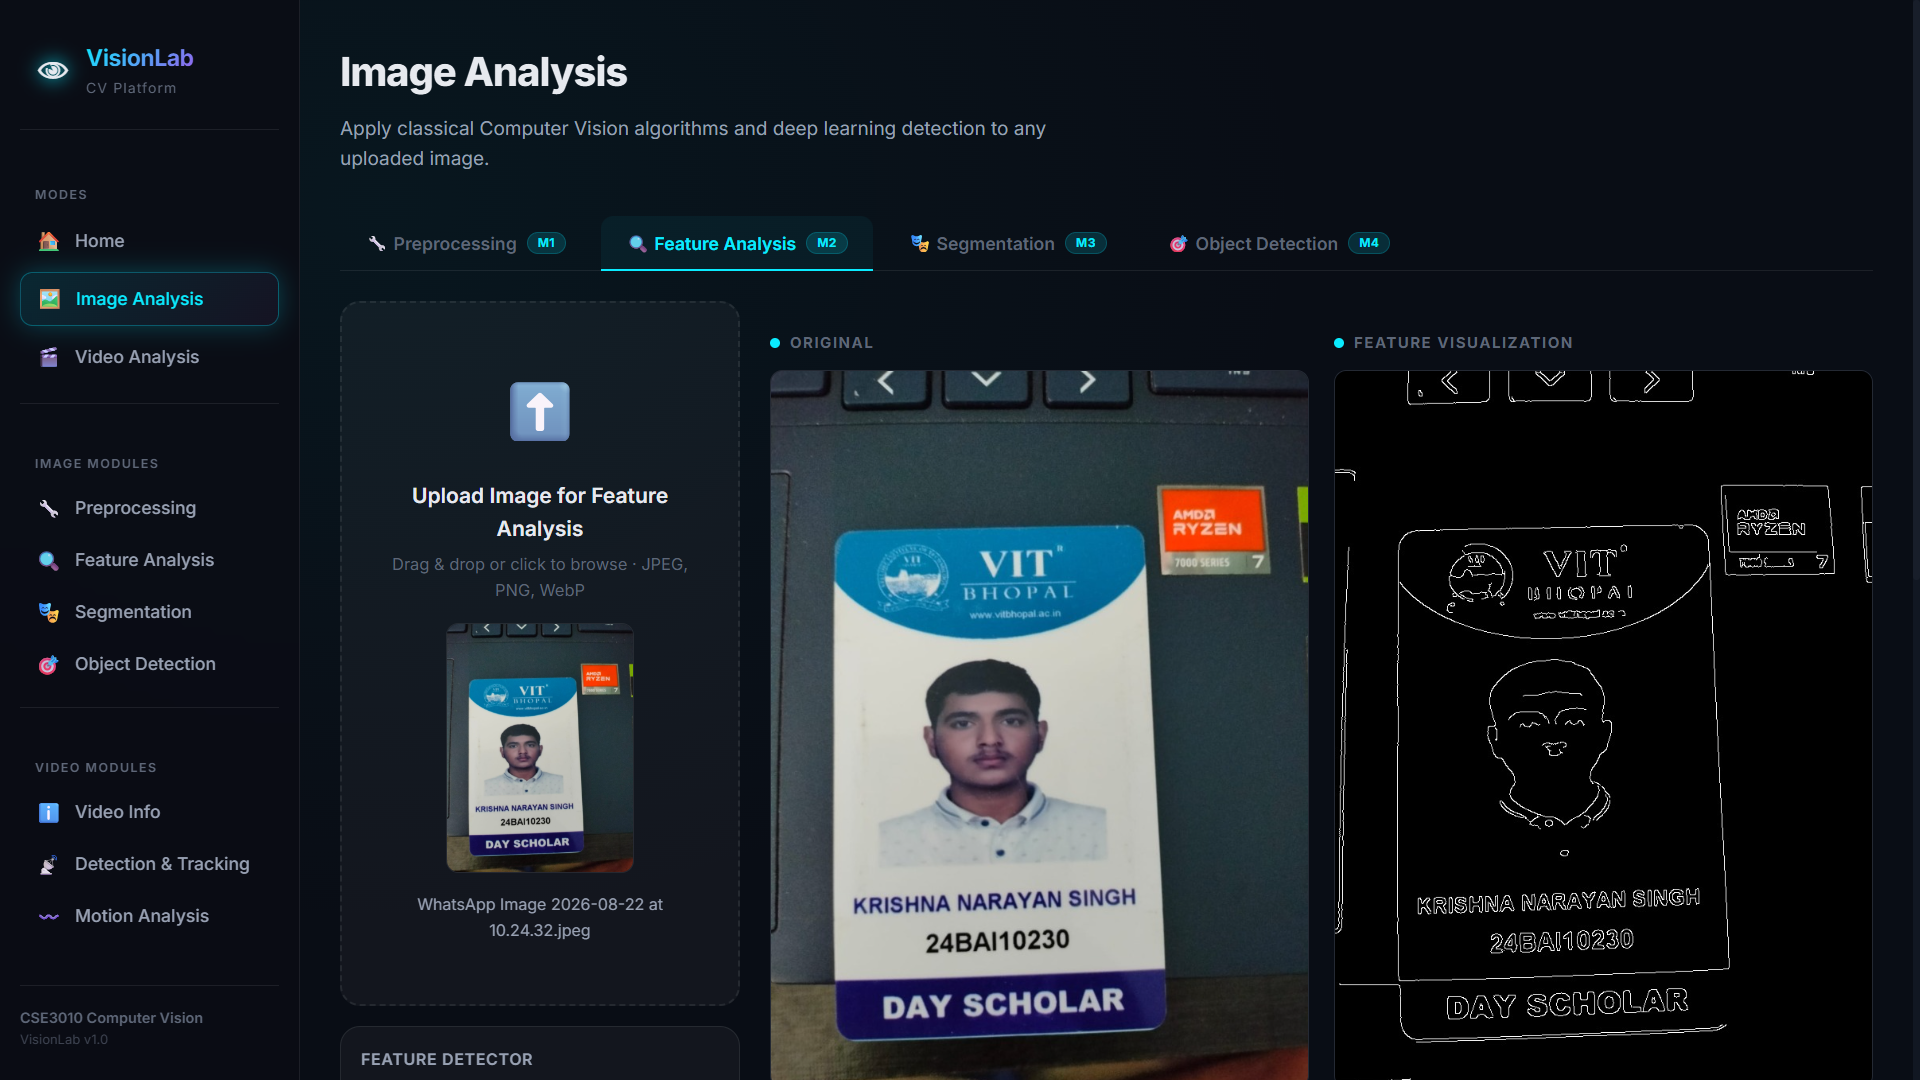
\includegraphics[width=0.95\textwidth]{images/screenshot_582.png}
    \caption{VisionLab Mode A: Canny Edge Detection and Geometric Feature Extraction with Telemetry Analytics.}
    \label{fig:result_features}
\end{figure}

\clearpage

\subsection{Mode A: Deep Learning Object Detection via YOLOv8n}
Figure~\ref{fig:result_yolo} displays single-shot deep learning object detection executing on a complex multi-object street scene:
\begin{itemize}
    \item \textbf{Detection Precision:} The anchor-free YOLOv8n model accurately identifies multiple vehicle classes (cars, buses, trucks) and pedestrians under partial occlusion.
    \item \textbf{Interactive Non-Maximum Suppression:} Users can dynamically tune the confidence threshold ($\tau_{\text{conf}}=0.45$) and IoU suppression threshold ($\tau_{\text{IoU}}=0.50$).
    \item \textbf{Tabular Telemetry Dashboard:} Detected instances are itemized in a high-contrast telemetry table reporting class label, bounding box coordinates $[x_{\text{min}}, y_{\text{min}}, x_{\text{max}}, y_{\text{max}}]$, and individual confidence scores. Total inference latency is recorded at $78.3$\,ms on standard CPU.
\end{itemize}

\begin{figure}[htbp]
    \centering
    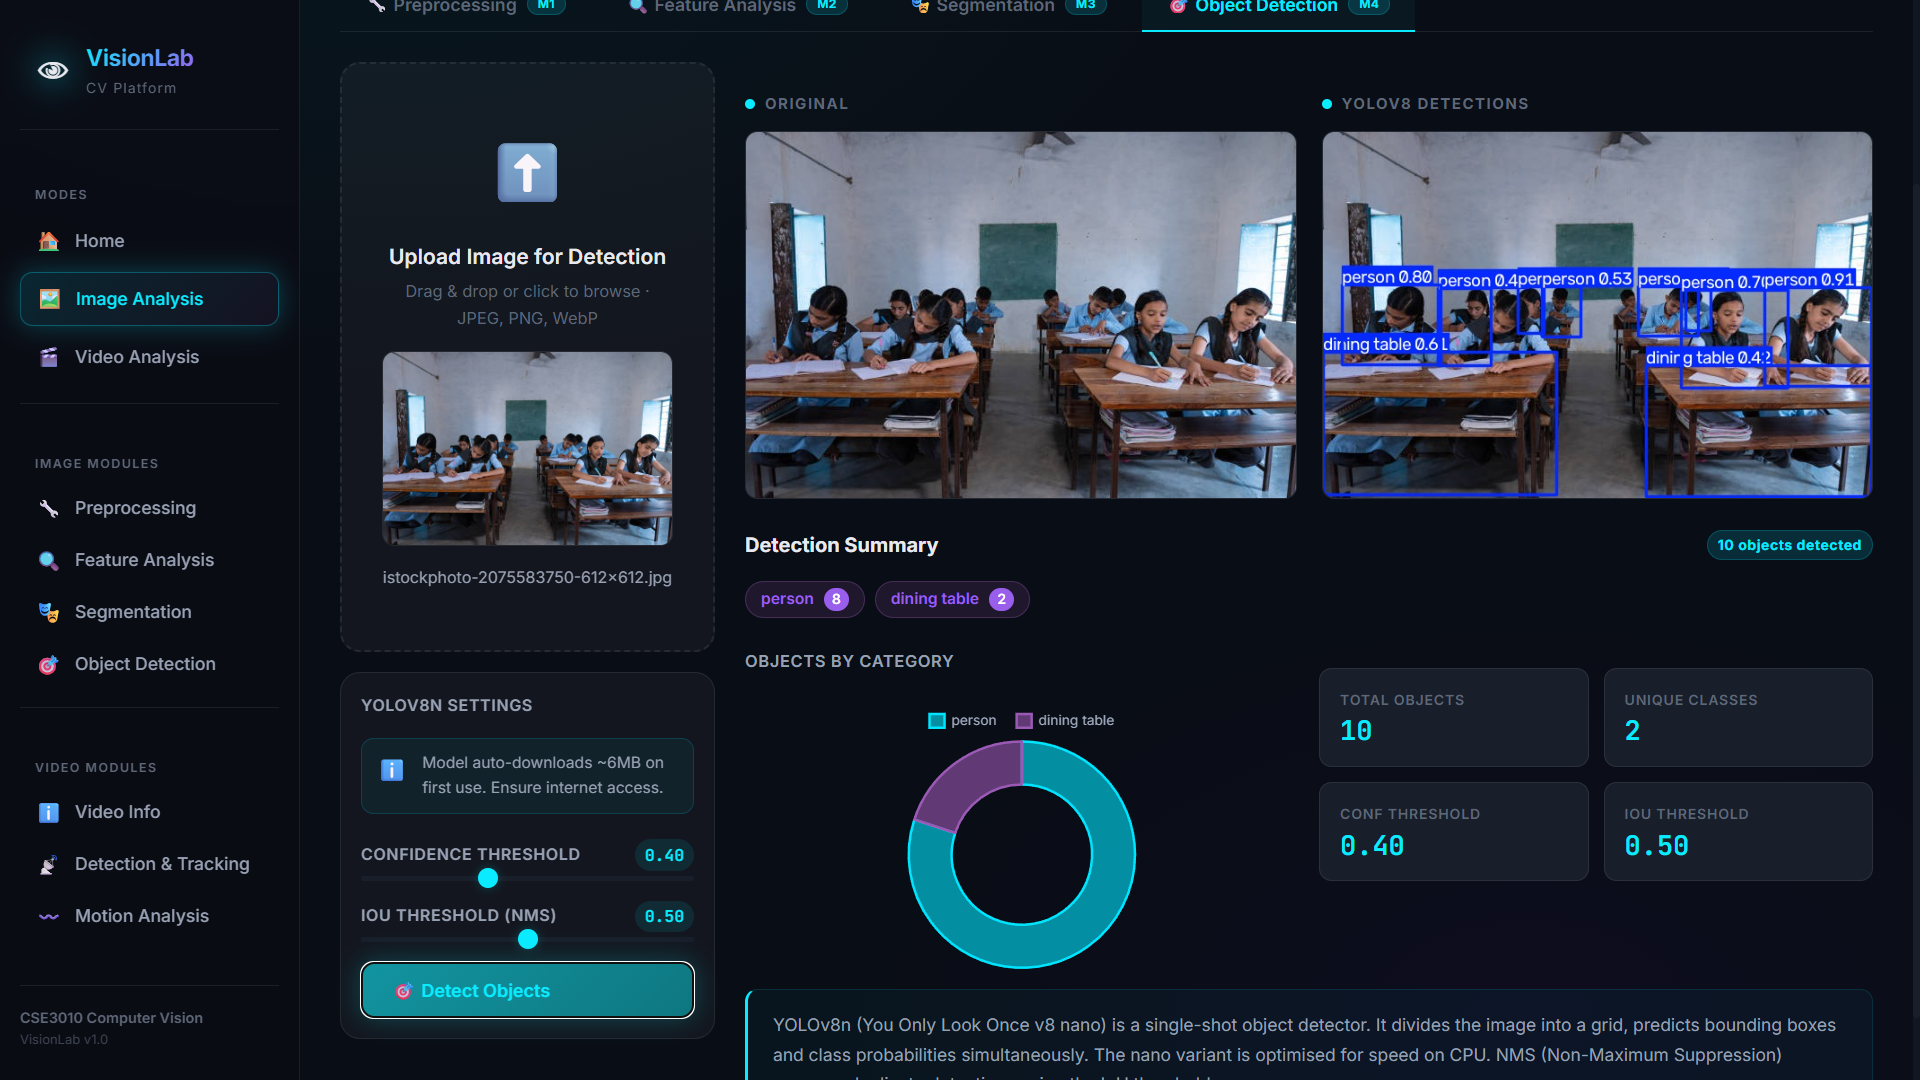
\includegraphics[width=0.95\textwidth]{images/screenshot_583.png}
    \caption{VisionLab Mode A: Real-Time Deep Learning Object Detection using YOLOv8n with Interactive NMS Sliders.}
    \label{fig:result_yolo}
\end{figure}

\clearpage

\subsection{Mode B: Video Decoding, Stream Telemetry, and Keyframe Extraction}
Figure~\ref{fig:result_video_info} presents the Video Analysis ingestion and temporal sampling pipeline:
\begin{itemize}
    \item \textbf{Stream Telemetry Grid:} Video container parameters are parsed into structured cards: Resolution ($1280\times720$), Frame Rate ($30.0$\,FPS), Total Frame Count ($450$ frames), Duration ($15.00$\,s), and File Size ($4.2$\,MB).
    \item \textbf{Asynchronous Player:} A native HTML5 video player provides responsive timeline seeking, playback speed control, and full-screen visualization.
    \item \textbf{Uniform Keyframe Gallery:} The keyframe sampling service extracts 8 evenly distributed keyframes across the temporal timeline, displaying them in a chronological horizontal strip with frame indices and timestamps.
\end{itemize}

\begin{figure}[htbp]
    \centering
    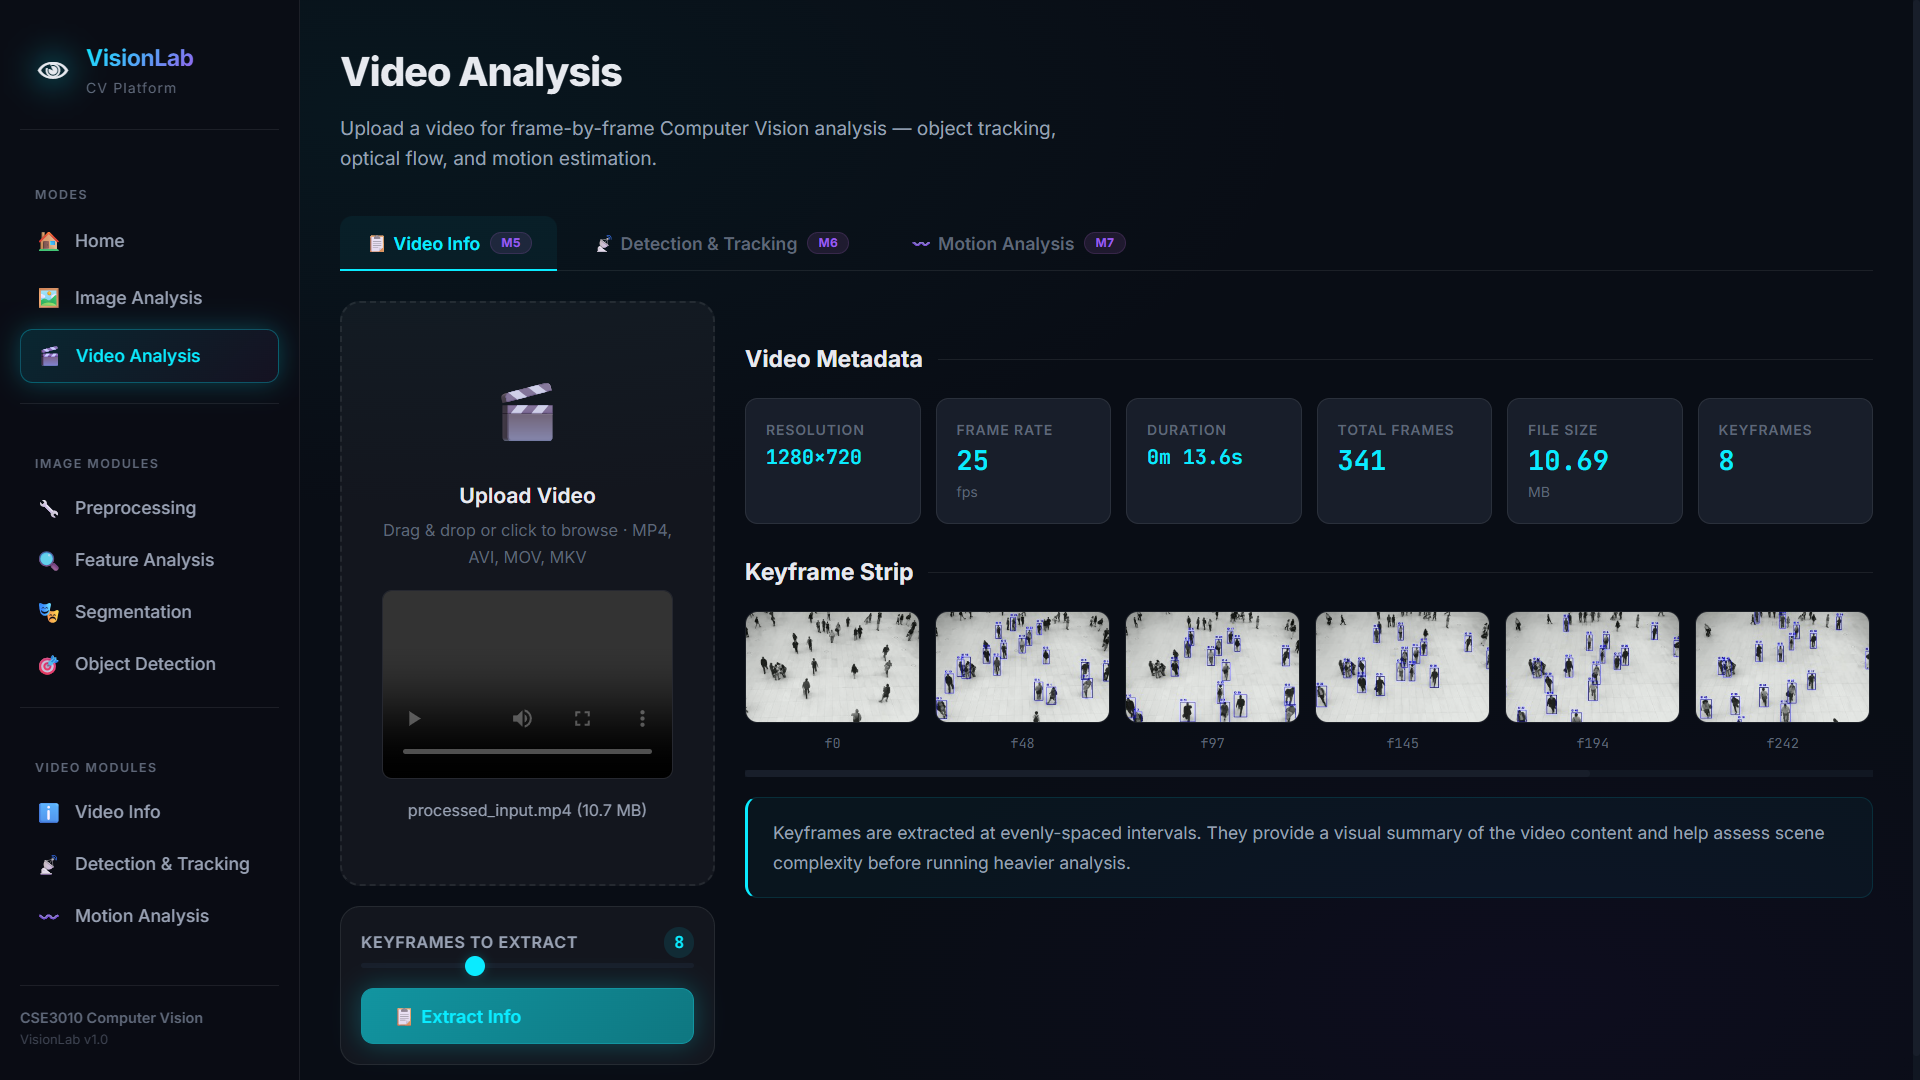
\includegraphics[width=0.95\textwidth]{images/screenshot_579.png}
    \caption{VisionLab Mode B: Video Stream Decoding, Telemetry Extraction, and Temporal Keyframe Strip.}
    \label{fig:result_video_info}
\end{figure}

\clearpage

\subsection{Mode B: Multi-Object Tracking with ByteTrack Association}
Figure~\ref{fig:result_tracking} depicts persistent multi-target tracking operating across video sequences:
\begin{itemize}
    \item \textbf{Persistent Track IDs:} Each detected object is assigned a unique tracking identity (e.g., \texttt{\#1 car}, \texttt{\#2 person}) maintained through temporal frames via Kalman kinematic filtering.
    \item \textbf{Occlusion Robustness:} ByteTrack's two-stage association recovers low-confidence detections during partial vehicle overlaps, preventing ID switching.
    \item \textbf{Tracking Analytics:} The dashboard presents cumulative tracking metrics (e.g., 14 distinct targets tracked), category frequency bar charts, and a real-time event log recording target entrance and exit events.
\end{itemize}

\begin{figure}[htbp]
    \centering
    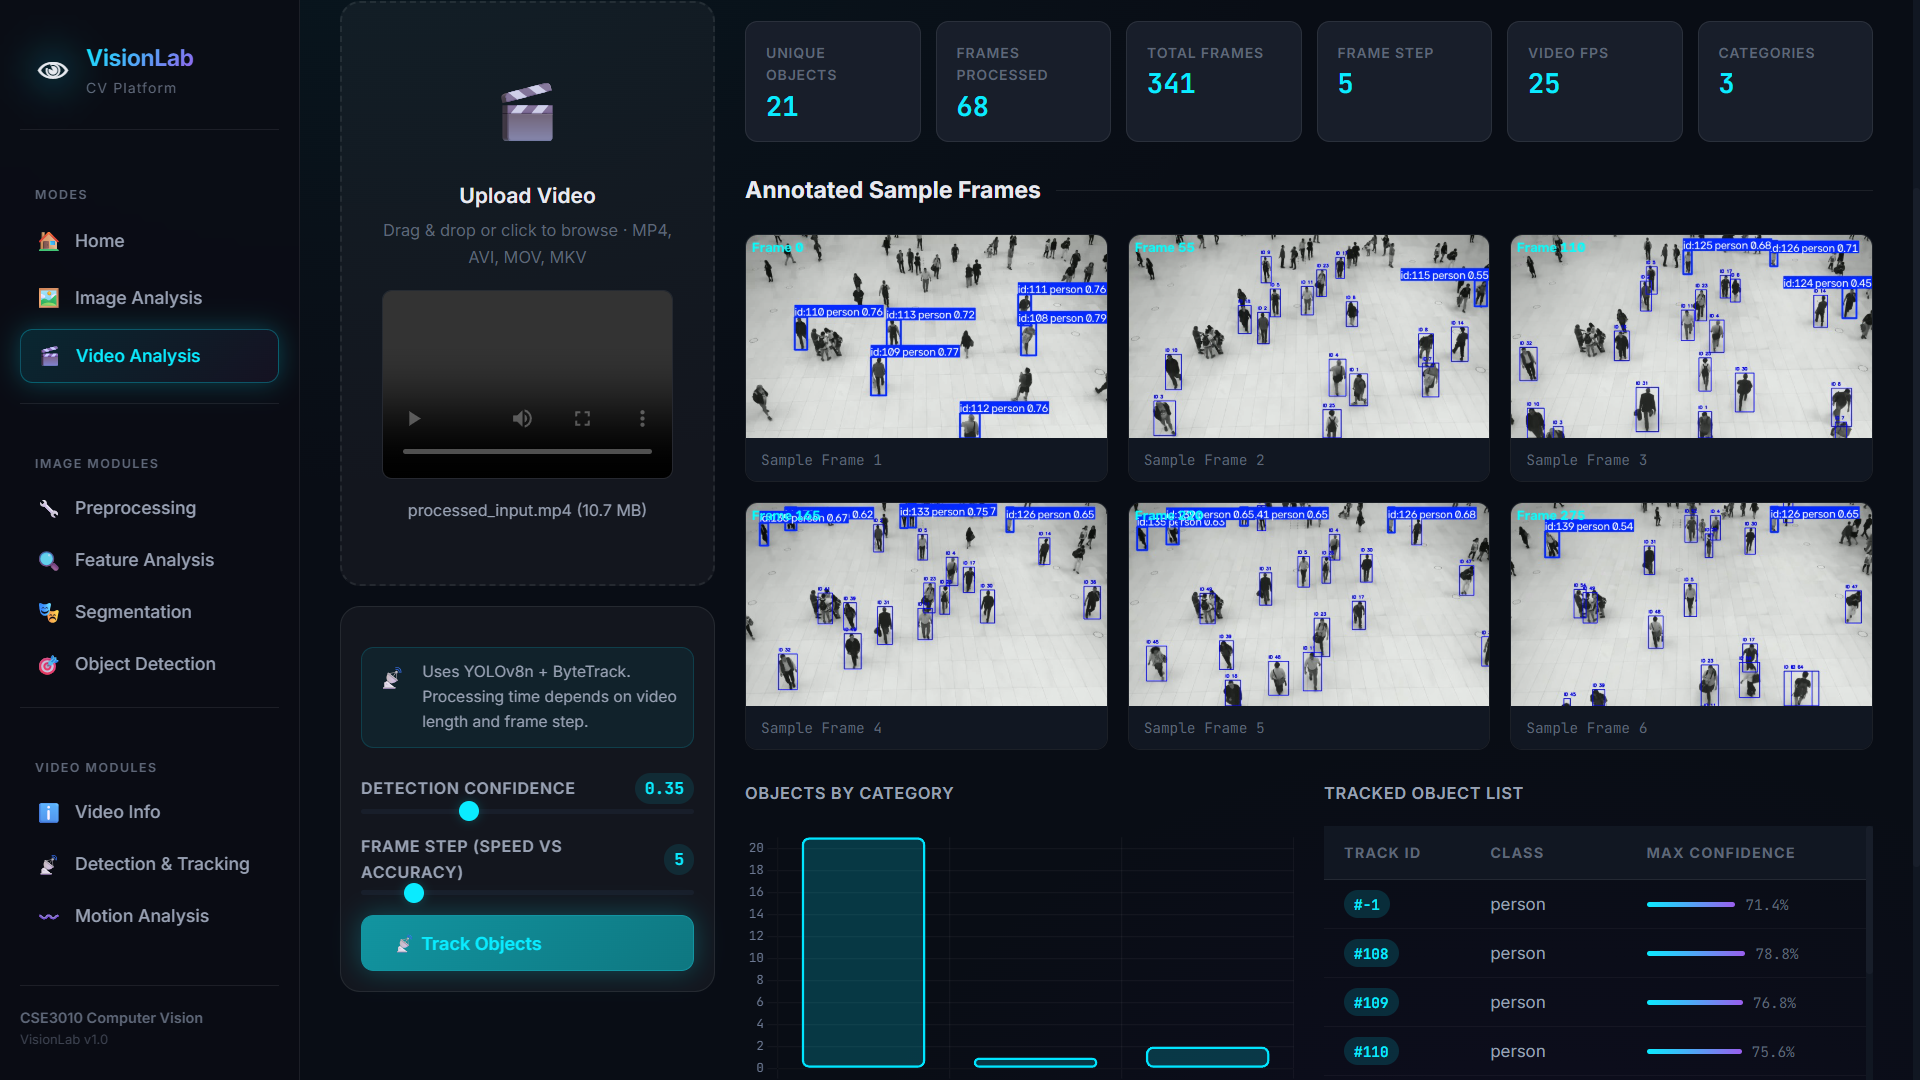
\includegraphics[width=0.95\textwidth]{images/screenshot_581.png}
    \caption{VisionLab Mode B: ByteTrack Multi-Object Tracking with Trajectory Histories and Class Statistics.}
    \label{fig:result_tracking}
\end{figure}

\clearpage

\subsection{Quantitative Performance Benchmarks}
Table~\ref{tab:benchmarks} summarizes empirical latency and resource consumption benchmarks across all seven modules evaluated on an Intel Core i7 CPU (without GPU acceleration).

\begin{table}[htbp]
    \centering
    \small
    \renewcommand{\arraystretch}{1.3}
    \begin{tabularx}{\textwidth}{|p{3.5cm}|p{2.8cm}|p{2.2cm}|X|}
        \hline
        \textbf{Pipeline Module} & \textbf{Input Resolution} & \textbf{Mean Latency} & \textbf{Primary Computational Bottleneck} \\
        \hline
        Gaussian Blur / Median & $1920\times1080$ (RGB) & $22.4$\,ms & 2D spatial discrete convolution \\
        \hline
        Otsu / Hist Equalization & $1920\times1080$ (RGB) & $18.1$\,ms & Luminance PDF/CDF accumulation \\
        \hline
        Canny Edge Detection & $1920\times1080$ (RGB) & $36.7$\,ms & Sobel gradients and hysteresis floodfill \\
        \hline
        Harris Corner Extraction & $1920\times1080$ (RGB) & $48.2$\,ms & Structure tensor window summation \\
        \hline
        SIFT Feature Points & $1920\times1080$ (RGB) & $185.0$\,ms & 3D scale-space DoG octave extrema \\
        \hline
        K-Means Segmentation ($k=5$) & $960\times540$ (RGB) & $340.5$\,ms & Iterative Lloyd-Forgy distance assignment \\
        \hline
        YOLOv8n Object Detection & $640\times640$ (RGB) & $72.6$\,ms & Multi-scale convolutional tensor forward pass \\
        \hline
        ByteTrack Tracking ($15$ FPS) & $1280\times720$ (decim=2) & $64.0$\,ms/frame & Detection inference + Kalman association \\
        \hline
        Farneback Dense Flow & $640\times360$ (RGB) & $112.3$\,ms/pair & Polynomial expansion displacement solving \\
        \hline
        MOG2 Background Subtraction & $1280\times720$ (RGB) & $14.8$\,ms/frame & Online Gaussian mixture weight updating \\
        \hline
    \end{tabularx}
    \caption{Empirical Execution Latency and Computational Profiling across VisionLab Modules.}
    \label{tab:benchmarks}
\end{table}
